\documentclass{article}
\usepackage[utf8x]{inputenc}
\usepackage{ucs}
\usepackage{amsmath} 
\usepackage{amsfonts}
\usepackage{upgreek}
\usepackage[english,russian]{babel}
\usepackage{graphicx}
\usepackage{float}
\usepackage{textcomp}
\usepackage{hyperref}
\usepackage{mathtools}
\usepackage{geometry}
  \geometry{left=2cm}
  \geometry{right=1.5cm}
  \geometry{top=1cm}
  \geometry{bottom=2cm}
\usepackage{tikz}
\usepackage{ccaption}
\usepackage{multicol}
%\setlength{\columnsep}{1.5cm}
%\setlength{\columnseprule}{0.2pt}
\usepackage{listings}

\DeclarePairedDelimiter\ceil{\lceil}{\rceil}
\DeclarePairedDelimiter\floor{\lfloor}{\rfloor}

\begin{document}
\pagenumbering{gobble}

\lstset{
  language=C,                % choose the language of the code
  basicstyle=\linespread{1.1}\ttfamily,
  columns=fixed,
  fontadjust=true,
  basewidth=0.5em,
  keywordstyle=\color{blue}\bfseries,
  commentstyle=\color{gray},
  stringstyle=\ttfamily\color{orange!50!black},
  showstringspaces=false,
  %numbers=false,                   % where to put the line-numbers
  numbersep=5pt,
  numberstyle=\tiny\color{black},
  numberfirstline=true,
  stepnumber=1,                   % the step between two line-numbers.        
  numbersep=10pt,                  % how far the line-numbers are from the code
  backgroundcolor=\color{white},  % choose the background color. You must add \usepackage{color}
  showstringspaces=false,         % underline spaces within strings
  captionpos=b,                   % sets the caption-position to bottom
  breaklines=true,                % sets automatic line breaking
  breakatwhitespace=true,         % sets if automatic breaks should only happen at whitespace
  xleftmargin=.2in,
  extendedchars=\true,
  keepspaces = true,
}
\lstset{literate=%
   *{0}{{{\color{red!20!violet}0}}}1
    {1}{{{\color{red!20!violet}1}}}1
    {2}{{{\color{red!20!violet}2}}}1
    {3}{{{\color{red!20!violet}3}}}1
    {4}{{{\color{red!20!violet}4}}}1
    {5}{{{\color{red!20!violet}5}}}1
    {6}{{{\color{red!20!violet}6}}}1
    {7}{{{\color{red!20!violet}7}}}1
    {8}{{{\color{red!20!violet}8}}}1
    {9}{{{\color{red!20!violet}9}}}1
}

\title{Семинар \#14: Безопасность и работа с файлами. Классные задачи.\vspace{-5ex}}\date{}\maketitle

\subsection*{Проверка на ошибки. Переменная \texttt{errno} и функция \texttt{perror}.}
При работе с функциями, которые взаимодействуют с операционной системой, такие как \texttt{malloc} или \texttt{fopen} нужно всегда предусматривать возможность возникновения ошибки. Так например, при вызове \texttt{malloc} заправшиваемого объёма памяти может не найтись или при вызове \texttt{fopen} файл с нужным названиям может не существовать. В этих случаях функции возвращают значени \texttt{NULL}.
\begin{lstlisting}
#include <stdio.h>
int main()
{
	FILE* file = fopen("input.txt", "r");
	if (file == NULL)
	{
		perror("Error");
		exit(1);
	}
	// Работаем с указателем file
	fclose(file);
}
\end{lstlisting}
При этом ошибка может быть разной. Например, при открытии файла ошибки могут быть такими: нет такого файла; неправильный режим открытия; файл есть, но нет прав доступа для работы с ним; файл является директорией и другие. Чтобы понять какая именно ошибка случилась, можно воспользоваться переменной \texttt{errno}, которая хранит в себе код последней ошибки. Пример в файле \texttt{0errno.c}. Если нужно просто распечатать сообщение о последней ошибке, то можно воспользоваться функцие \texttt{perror}. Пример в файле \texttt{1perror.c}.
\begin{itemize}
\item Напишите программу, которая будет проверять существует ли файл. (Если файл не существует, то переменная \texttt{errno} будет равна константе \texttt{ENOENT}).
\end{itemize}

\subsection*{Опасность функций семейства \texttt{scanf} при считывании строк.}
Функции \texttt{scanf}, \texttt{fscanf} и \texttt{sscanf} имеют одну неприятную особеность при считывании строк. Спецификатор \texttt{\%s} делает следующее: считывает строку и записывает её всю по передаваемому ей адресу. Это может привести к серьёзным ошибкам если то место, куда мы записываем строку будет меньше, чем записываемая строка. Рассмотрим, например, следующую простую программу:
\begin{lstlisting}
#include <stdio.h>
int main()
{
	char a[5] = "Lion";
	char b[5];
	
	scanf("%s", b);
	printf("a = %s\n", a);
	printf("b = %s\n", b);
}
\end{lstlisting}
\begin{itemize}
\item Что напечатает эта программа, если на вход передать строку \texttt{Cat}?
\item Что напечатает эта программа, если на вход передать строку \texttt{Zebra}?
\item Что напечатает эта программа, если на вход передать строку \texttt{Elephant}?
\item Как исправить ошибки?
\end{itemize}

\begin{center}
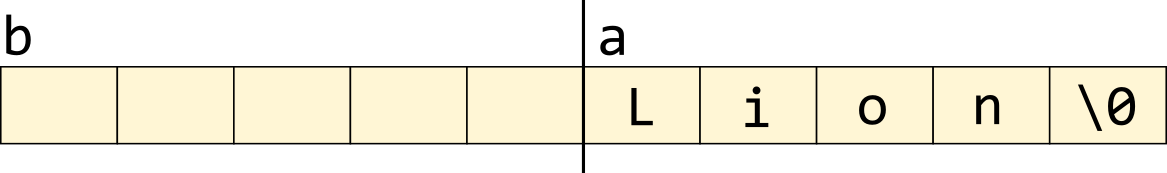
\includegraphics[scale=1]{../images/scanf_safety.png}
\end{center}

Функция \texttt{scanf} выходит за границы массива \texttt{b} и переписывает другую строку. Если бы на месте строки \texttt{a} была бы переменная другого типа, то \texttt{scanf} испортил бы и её. Более того, таким поведением \texttt{scanf} могут воспользоваться злоумышленники и взломать вашу программу.

\subsection*{Функция \texttt{fgets}.}
Таким образом функция \texttt{scanf} со спецификатором \texttt{\%s} является небезопасной. Чтобы недопустить подобных ошибок лучше использовать функцию \texttt{fgets}:
\begin{verbatim}
fgets(<адрес куда записываем>, <вместимость строки куда записываем>, <файловый указатель или stdin>)
\end{verbatim}
Функция \texttt{fgets} считывает строку до символа \texttt{\textbackslash n} либо пока не закончится место. В конце файла функция \texttt{fgets} возвращает \texttt{NULL}. Таким образом пример выше перепишется в виде:
\begin{lstlisting}
#include <stdio.h>
int main()
{
	char a[5] = "Lion";
	char b[5];
	
	fgets(b, 5, stdin);
	printf("a = %s\n", a);
	printf("b = %s\n", b);
}
\end{lstlisting}

\begin{itemize}
\item Что напечатает эта программа, если подать на вход строки \texttt{Cat}, \texttt{Zebra} или \texttt{Elephant}?
\item Напишите программу, которая печатает всё содержимое файла на экран с помощью функции \texttt{fgets} в предположение, что строка файла не больше 200 символов. Выведите на экран содержимое файла \texttt{sail.txt}.
\end{itemize}

\subsection*{Функция \texttt{fgetс}.}
Функция \texttt{fgetc} считывает 1 символ и возвращает код \texttt{ASCII} символа или \texttt{EOF} если дошли до конца файла (\texttt{EOF} это просто константа равная -1). Пример считывания:

\begin{lstlisting}
#include <stdio.h>
int main()
{
    FILE* f = fopen("test.txt", "r");
    while (1)
    {
        // Считываем 1 символ
        int c = fgetc(f);
		
        // Если он равен EOF, то выходим из цикла
        if (c == EOF)
            break;
            
        printf("%c\n", c);
	}
    fclose(f);
}
\end{lstlisting}

\begin{itemize}
\item Напишите программу, которая печатает количество строк в файле.
\item Напишите программу, которая печатает размер самой длинной строки файла.
\end{itemize}

\subsection*{Функции \texttt{ftell} и \texttt{fseek}.}

Процесс считывания файла можно представить как перемещение по набору байт. При открытии файла указатель положения равен нулю. При считывании он увеличивается на количество считанных байт.
\begin{center}
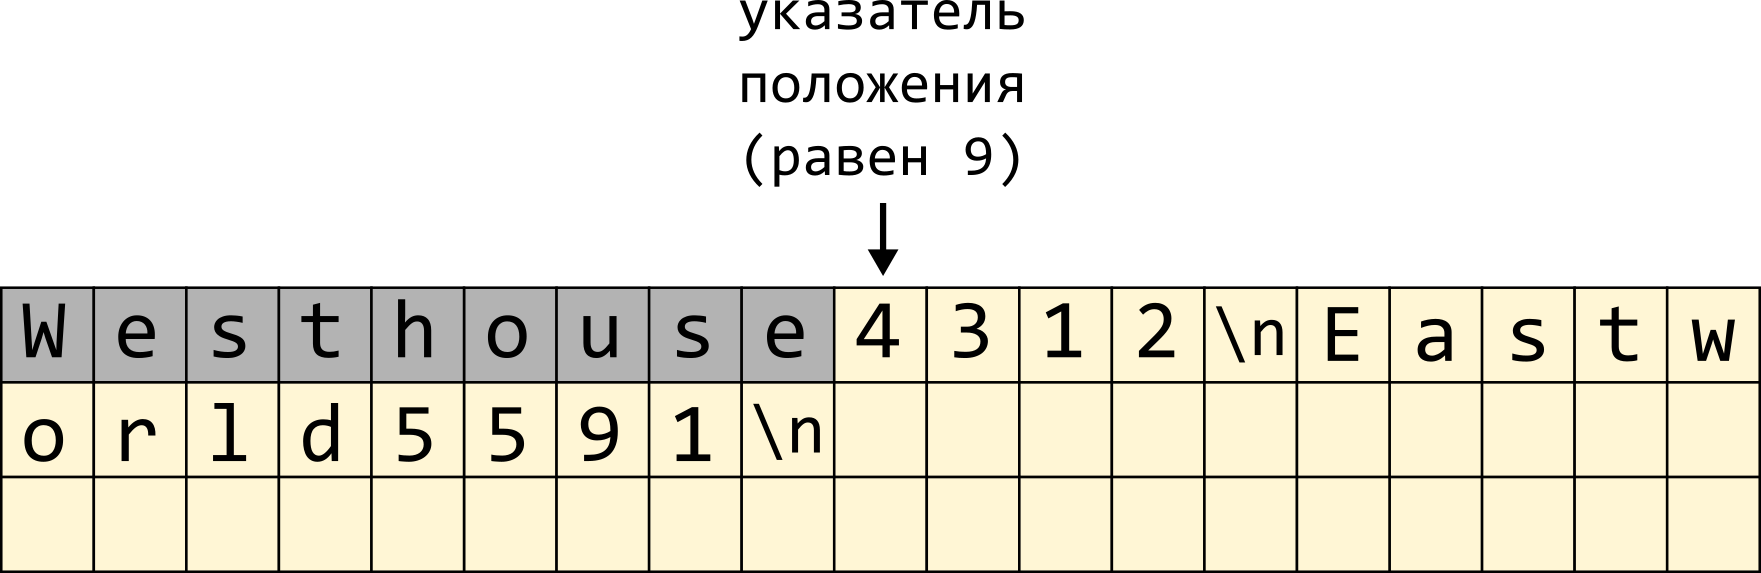
\includegraphics[scale=0.8]{../images/positioninfile.png}
\end{center}

Однако, положение в файле можно менять и без считывания при помощь функции \texttt{fseek}:
\begin{verbatim}
fseek(<файловый указатель>, <смещение>, <начало отсчёта>)
\end{verbatim}
Начало отсчёта в этой функции может принимать 3 значения:
\begin{enumerate}
\item \texttt{SEEK\_SET} -- отсчитывать от начала файла
\item \texttt{SEEK\_CUR} -- отсчитывать от текущего положения
\item \texttt{SEEK\_END} -- отсчитывать от конца файла
\end{enumerate}

Например:
\begin{lstlisting}
#include <stdio.h>
int main()
{
    FILE* f = fopen("test.txt", "r");
    fseek(f, 10, SEEK_SET); // Перемещаемся на 11 - й символ
    fseek(f, -1, SEEK_END); // Перемещаемся к последнему символу
	
    fseek(f, -1, SEEK_CUR); // Перемещаемся на 1 символ назад
    fseek(f, 0, SEEK_SET);  // Возвращаемся к началу
    fclose(f);
}

\end{lstlisting}

Функция \texttt{ftell(<файловый указатель>)} возвращает целое число -- текущее положение в файле.

\begin{itemize}
\item Написать программу, которая будет печатать 3 последних символа в файле.\\
\item Написать программу, которая будет считывать файл \texttt{test.txt} и печатать число, которое начинается с 10-го символа.
\item Написать программу, которая будет принимать название файла через аргумент командной строки и печатать его размер в байтах.\\
\textit{Подсказка:} Используйте \texttt{fseek}, чтобы перейти в конец файла и \texttt{ftell}, чтобы узнать позицию.

\item В файле \texttt{numbers.txt} хранятся некоторые целые числа (но не указано их количество). Напишите программу, которая будет считывать все числа из этого файла и печатать их на экран. Есла в файле содержится какие-то другие символы кроме цифр и пробельных символов, то программа должна печатать \texttt{Error!} и завершаться.\\
\textit{Подсказка:} Для начала нужно узнать количество чисел. Это можно сделать, используя \texttt{fgetc}. Затем считываем. Память для чисел выделяем в куче, так как их количество изначально неизвестно и может быть болишим.
\end{itemize}
\end{document}
